\newpage
\section{Recurrent Neural Networks}
\subsection{Processing Sequences}
So far, all the deep neural networks that we studied (MLPs, CNNs) had the same \emph{feed-forward} global structure: the network receives an input of fixed size, which is fed into the successive layers of the network, which produces a fixed-size output. This is known as a \emph{one-to-one} model, and is mostly used for image classification.

When considering other applications, we would like more flexibility on the input and output sizes. For image captioning, we would like a \emph{one-to-many} model, where the input is a fixed size image, and the output a sentence of variable length. For text classification, such as sentiment analysis, we would like a \emph{many-to-one} model, where the input is a sentence of variable length and the output a fixed-size vector of class probabilities. Finally, we might want both the input and output to be variable in length, for instance in the case of machine translation: this requires a \emph{many-to-many} model.

\begin{figure}[H]
    \centering
    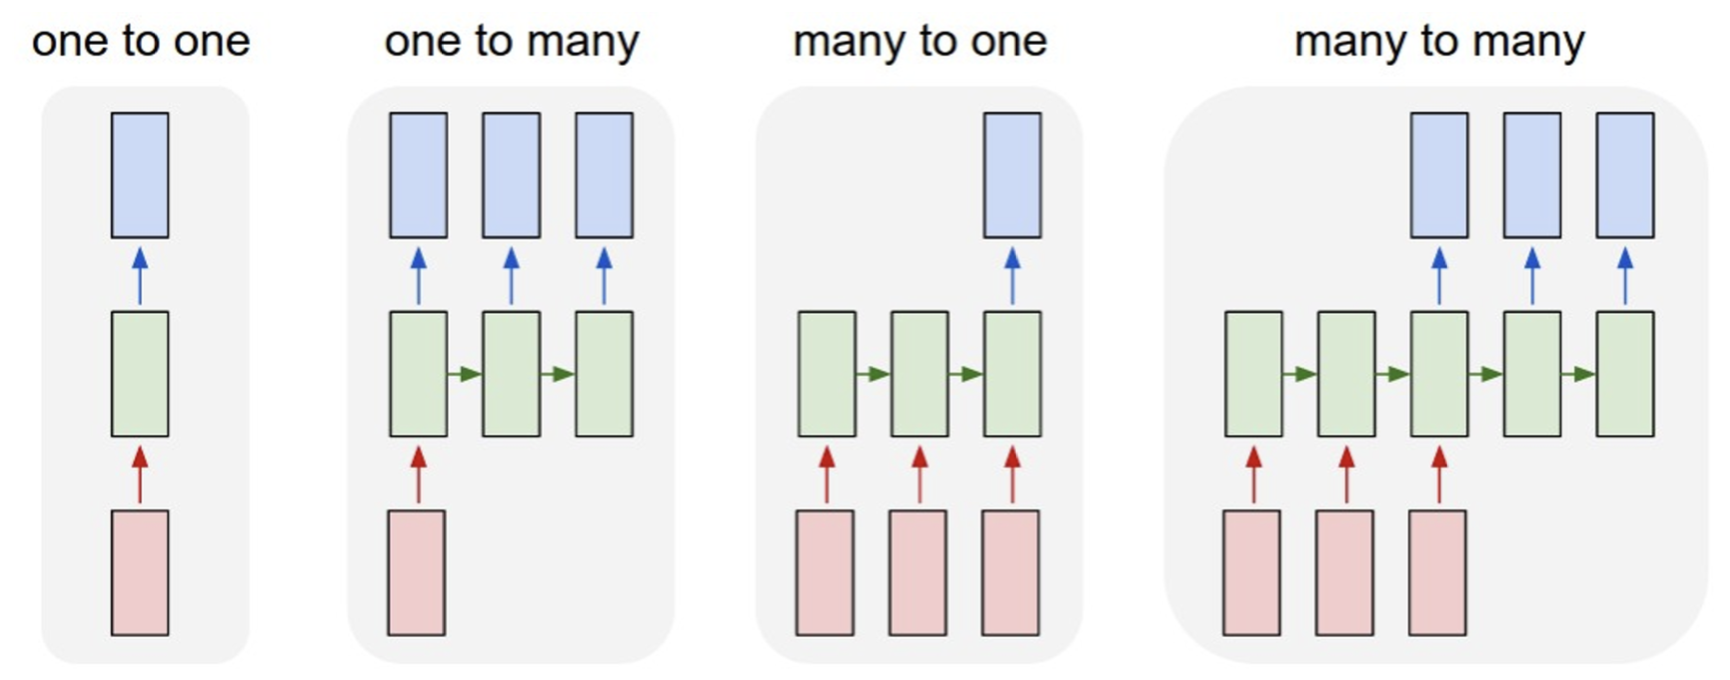
\includegraphics[width=.8\textwidth]{images/sequences.png}
\end{figure}

\emph{Recurrent Neural Networks} (RNNs) is a general paradigm which allows to handle all these different setups.

\subsection{Simple Recurrent Neural Network}
\subsubsection{General form}
\begin{wrapfigure}{r}{0.2\textwidth}
    \centering
    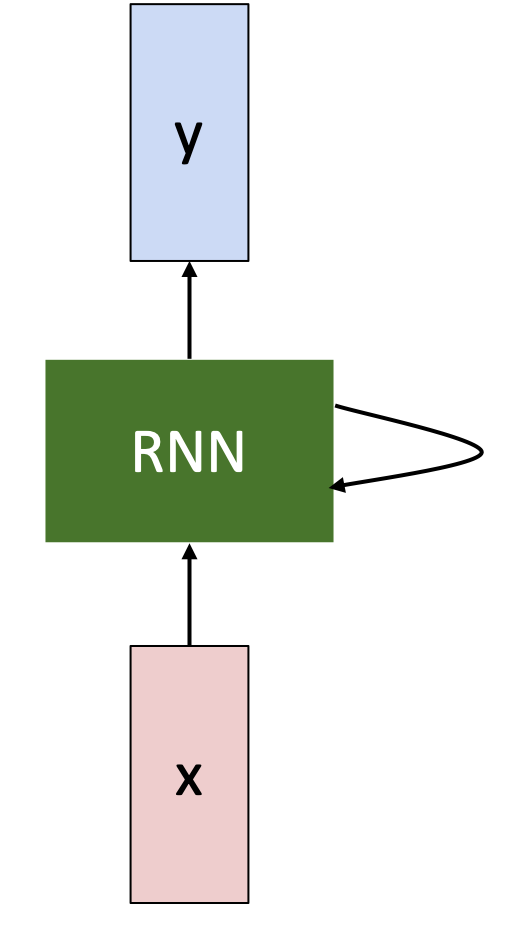
\includegraphics[width=.2\textwidth]{images/vanilla-rnn.png}
    \caption{A simple RNN.}
\end{wrapfigure}
In its simplest form, a Recurrent Neural Network posesses an internal hidden state which is updated each time that it reads an input. The handling of a sequential input (for instance, a sentence) follows this update loop: a fixed-size bit of the input is fed into the network, and is combined with the internal hidden state to produce an output and update the state. The next bit of the input is then fed to the network, and so on. 

Formally, this can be written as a recurrence relationship:
\begin{equation*}
    h_t = f_\theta(h_{t-1}, x_t)
\end{equation*}
where $x$ is a sequence of vectors, $(h_t)_t$ is the sequence of hidden states, and $f_\theta$ is our network depending on some parameter $\theta$. To produce an output at each time step, we can simply transform the hidden state into an ouput using a feed-forward neural network:
\begin{equation*}
    y_t = g_{\theta'}(h_t)
\end{equation*}
Note that the same functions $f, g$ and the same parameters $\theta, \theta'$ are used at each step, only the internal state changes.

\subsubsection{A vanilla RNN}
We can create a simple RNN built around a single hidden vector $h_t$:
\begin{equation*}
    \begin{aligned}
        h_t &= \tanh\left(W_h h_{t-1} + W_x x_t\right)\\
        y_t &= W_y h_t
    \end{aligned}
\end{equation*}

\subsubsection{Computational graphs of RNNs}
Alongside with this intuition of RNNs as networks with hidden cells, it is also useful to think of RNNs as computational graphs. The graph of an RNN can be unfolded over multiple time steps, expliciting the inputs and gradient flow.
\begin{figure}[H]
    \centering
    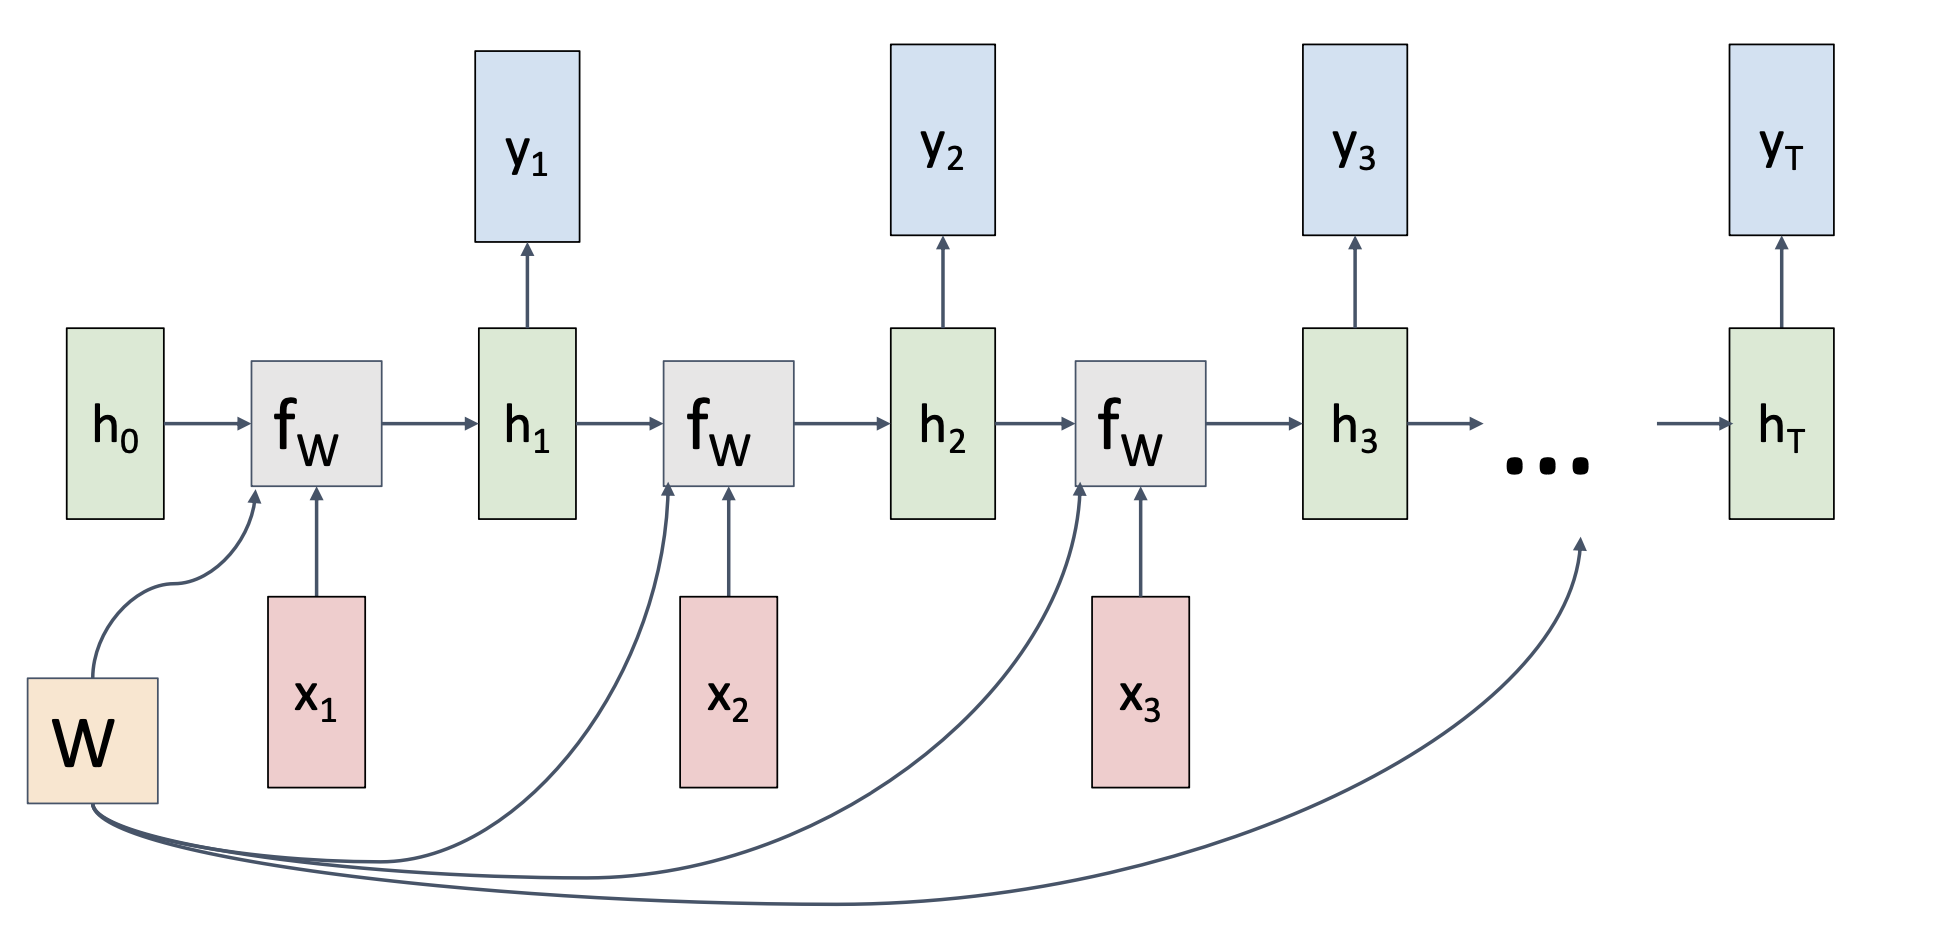
\includegraphics[width=.7\textwidth]{images/rnn-graph.png}
    \caption{Unfolded computation graph of an RNN.}
\end{figure}
The initial hidden state $h_0$ is often initialized to 0 in most contexts. It is then fed to the $f_\theta$ function with the first input $x_1$, which produces the new hidden state $h_1$. This hidden state can be used to compute the output $y_1$.

Note that the parameter $\theta$ remains the same for all; when computing the gradient $\frac{\partial\L}{\partial\theta}$, we will sum all the graidents coming from each time step to compute the 

\newpage